\subsection{Test framework}
As discussed in previous sections, the model is to be used as a state observer for the Hi-Fi simulation. The model was reduced from 10 to 8 states in \cref{sec:kalman}. The reduced order model will be referred to as the control model. \\

\noindent The control model must initially be tested to accurately estimate the observable states of the full 10-state model. In the test framework, the two models run in parallel, with the control signals $u$ equally applied to both systems. The control signals are computed by the controller K, based on the states of the control model. This framework is seen in \cref{fig:sim_modelSS_obs}. \\

\noindent As described in \cref{sec:observer-gain} a Luenberger observer gain $L$ was calculated. Any error between the actual output and estimated output will be multiplied by $L$ and added to the $\dot{\hat{x}}$. If $A-LC$ is stable, this topology will ensure $\hat{y}$ converges to $y$. If the states are observable (which the Kalman Decomposition ensures) and there is no present disturbance then $\hat{x}$ will converge to $x$. If a disturbance is present, the proportional observer gain will not be sufficient to estimate the states, and integral action should be included. For the purpose of these tests however, the error introduced by the disturbance is not handled by integral observer action. \\

\noindent For this test, the ambient temperature is set to 20$^{\circ}$C, which is its operating point value, such that no disturbance is present. This is clear by recalling that $\tilde{d} = d-d_o$. All states are initialized to the arbitrary value 1 to verify that all states are driven to zero and that the observed state vector $\hat{x}$ converges to $x$. It is recalled that in this coordinate system $x=0$ means $x-x_o = 0 \rightarrow x=x_o$. The control signal u is defined as $u=K\hat{x}$.

\begin{figure}[h!]
	\centering
	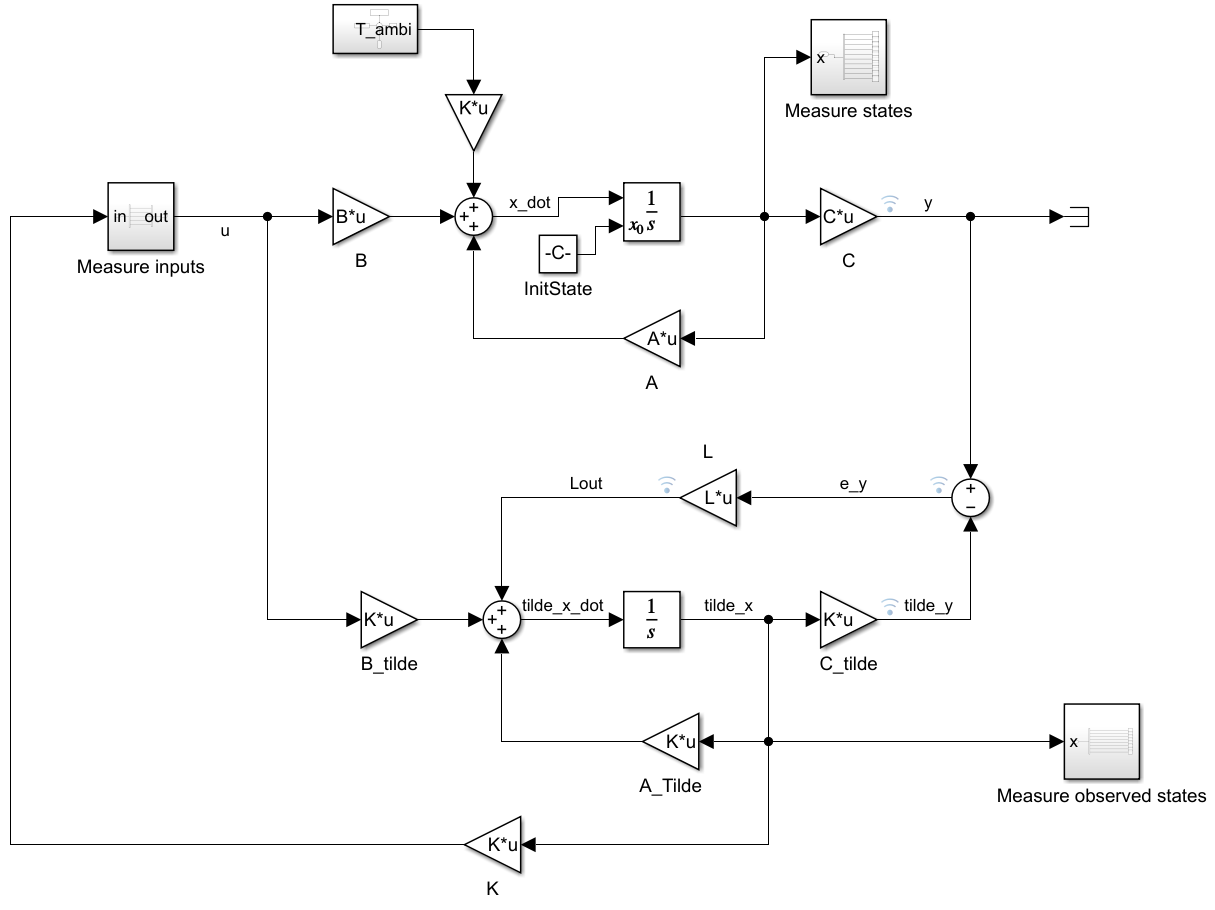
\includegraphics[width=1\textwidth]{Graphics/fig_modelSS_obs.png}
	\caption{The Matlab Simulink simulation model of the linearised system with feedback from Kalman Decomposition observer}
	\label{fig:sim_modelSS_obs}
\end{figure}

\newpage
\subsection{Test results}
The simulation was run for 10 hours to ensure that all states had settled. Four plots are made. In \cref{fig:sim_stateInput10h} a plot containing the states and inputs is seen. All states except the box temperature converge to steady state inside about half an hour. The box temperature settles after about 8-9 hours. It is also observed that the inputs stay inside a reasonable interval.

\begin{figure}[h!]
	\centering
	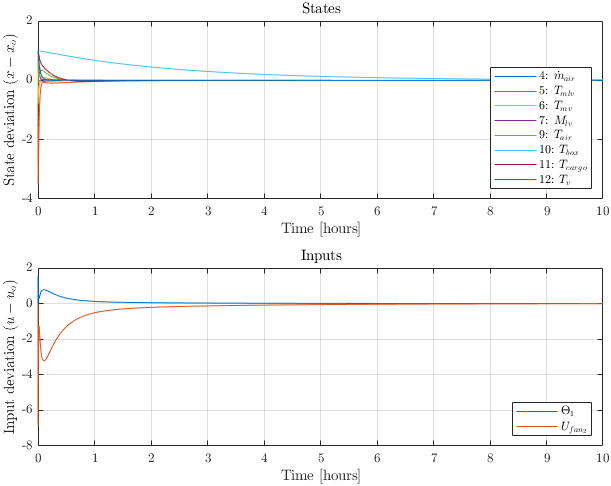
\includegraphics[width=00.7\textwidth]{Graphics/fig_stateInput10h.png}
	\caption{States and inputs plotted for 10 hours. All states settle within an hour except the box temperature which settles in about 7-8 hours}
	\label{fig:sim_stateInput10h}
\end{figure}

\newpage
\noindent In \cref{fig:sim_stateInput1h} the same plot as previously is seen but zoomed in at 1 hour such that the behavior of the states is more easily observed.

\begin{figure}[h!]
	\centering
	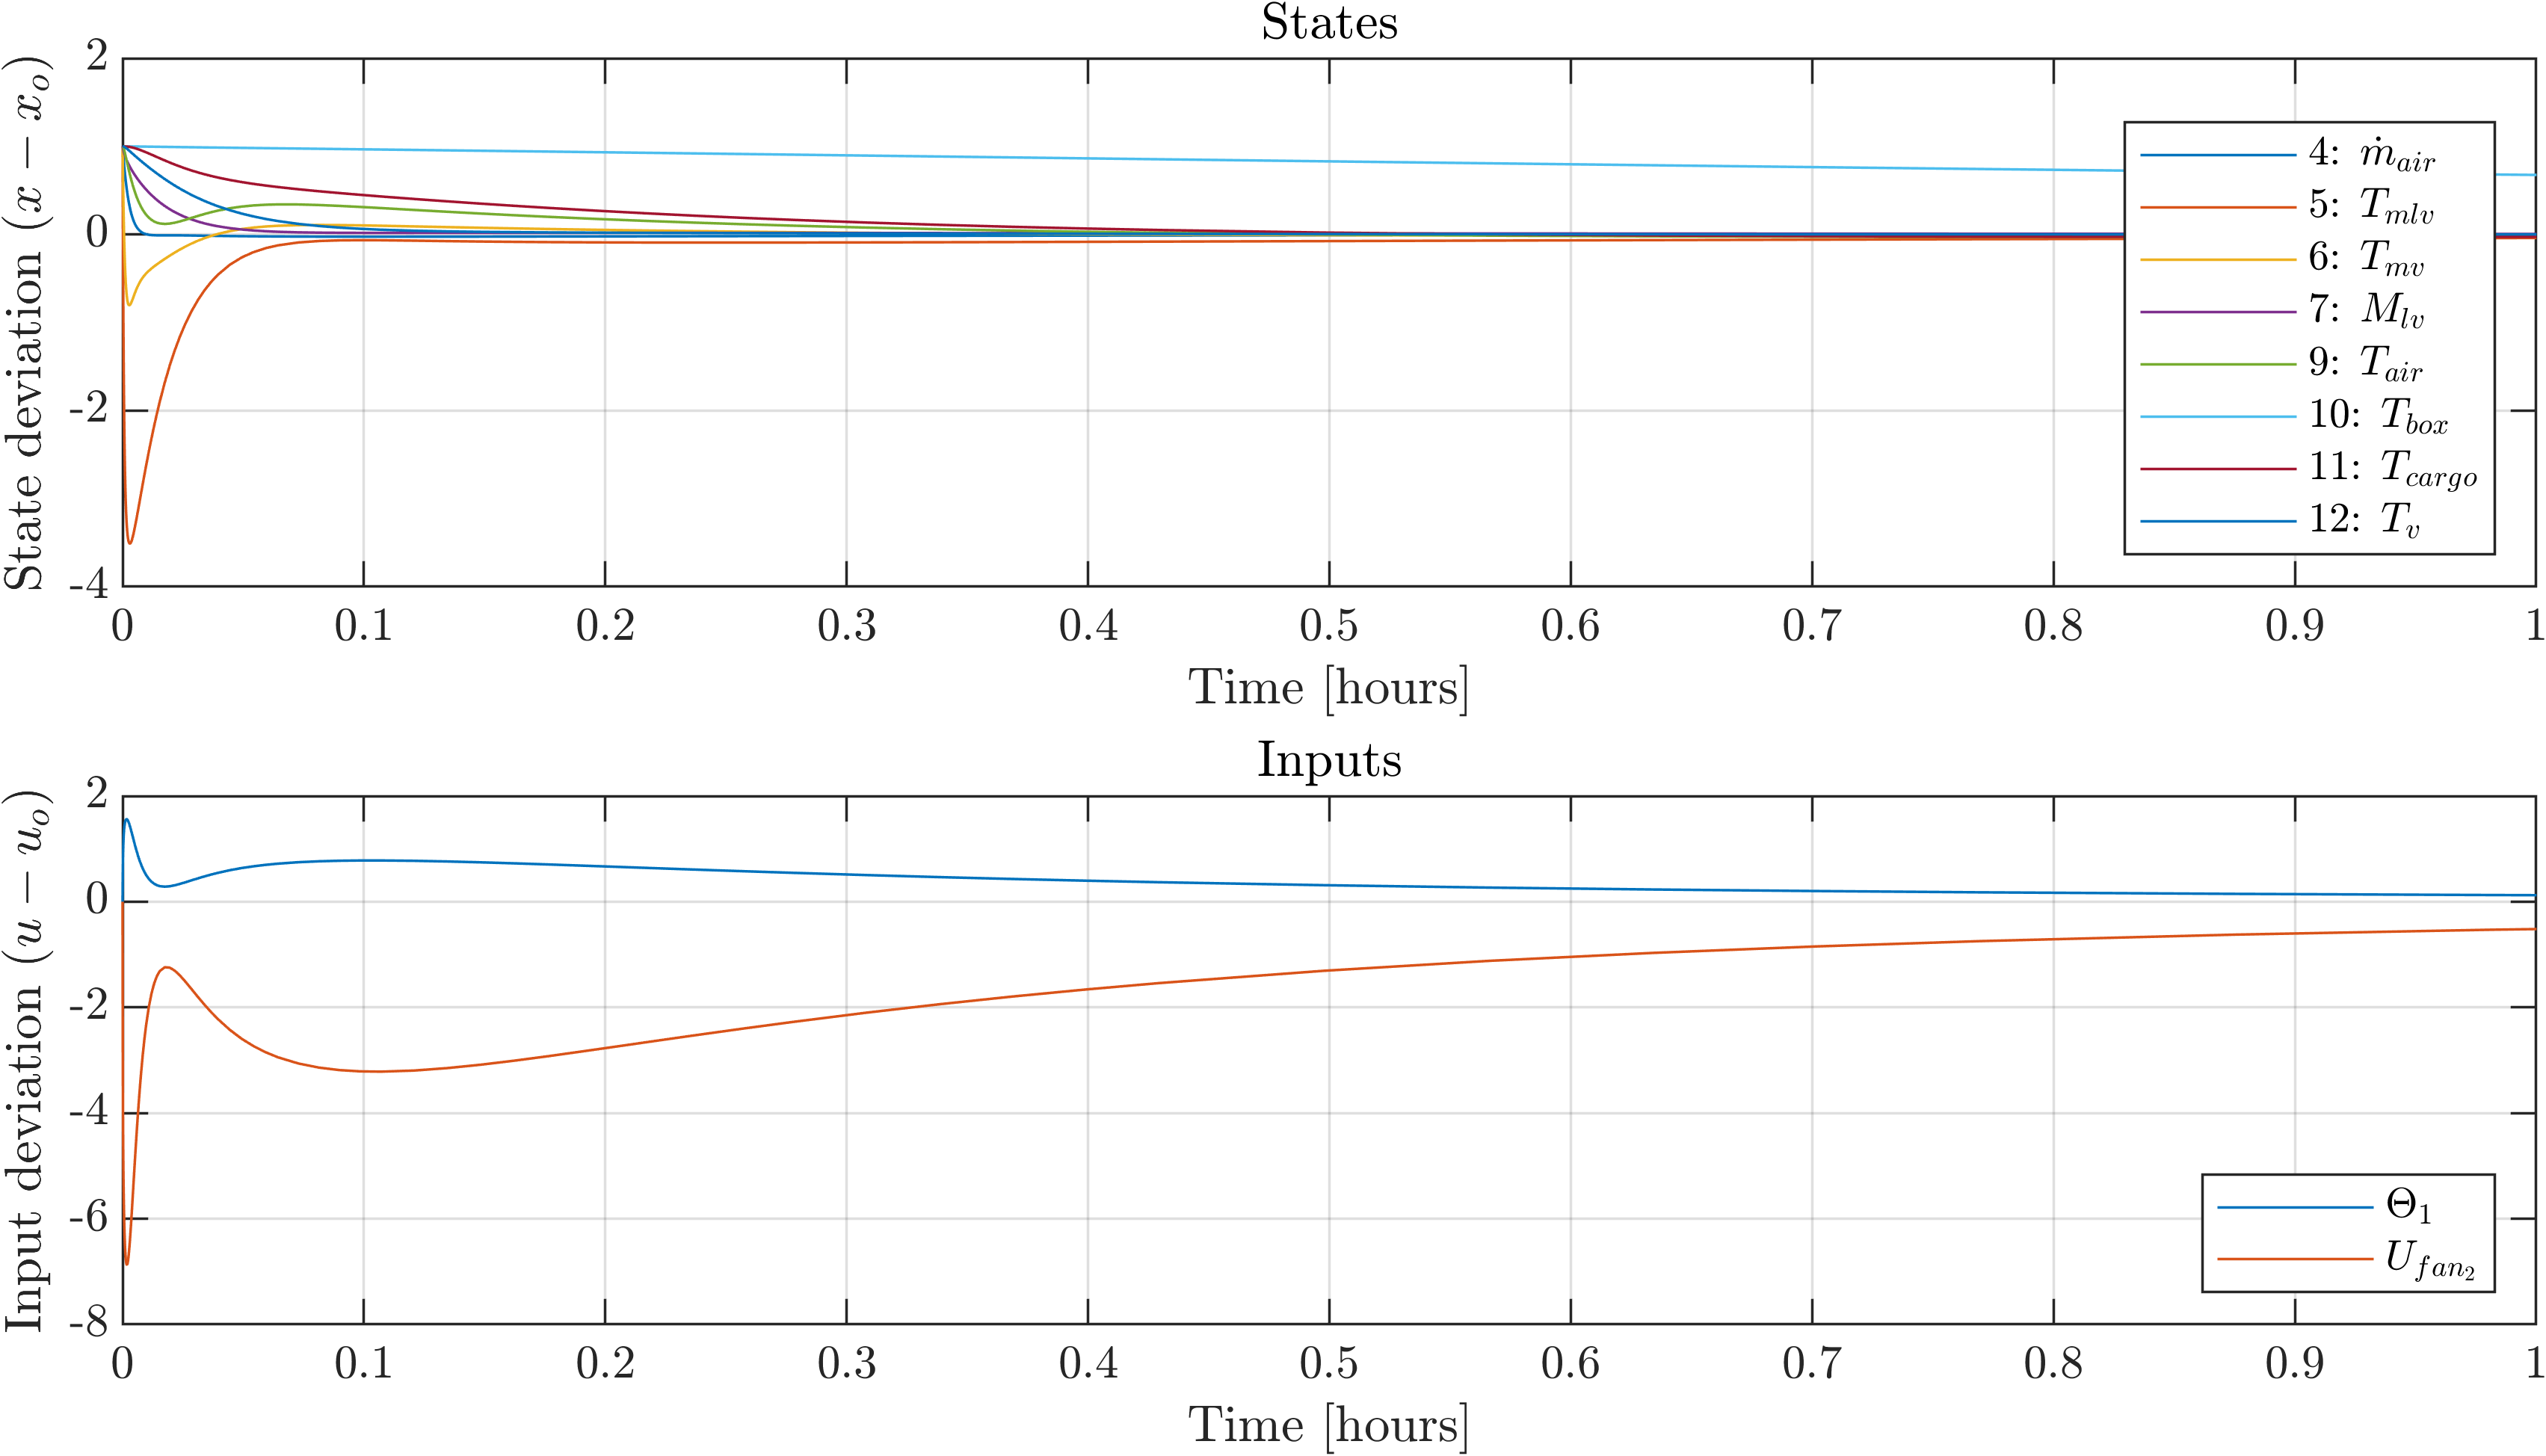
\includegraphics[width=0.66\textwidth]{Graphics/fig_stateInput1h.png}
	\caption{States and inputs plotted for 1 hour.}
	\label{fig:sim_stateInput1h}
\end{figure}


\noindent In \cref{fig:sim_stateObsState1h} the states are compared to the observed states, during the first hour of the simulation. It is seen that the observed states settle onto the actual states in around 0.1 hours.

\begin{figure}[h!]
	\centering
	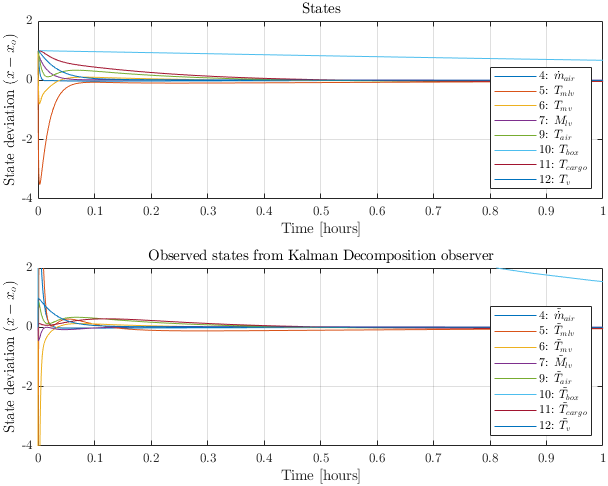
\includegraphics[width=0.66\textwidth]{Graphics/fig_stateObsState1h.png}
	\caption{States and Kalman Decomposition observed states plotted for 1 hour. The estimated box temperature obviously deviates but begins to settle towards the correct state value.}
	\label{fig:sim_stateObsState1h}
\end{figure}

\newpage
\noindent In \cref{fig:sim_stateObsState002h} further zoom is made on the time axis to observe the fast transients in the first seconds of the simulation where the observer converges from the big starting error. It can be seen that the observed states initially in the first seconds deviate greatly before settling close to the actual states.

\begin{figure}[h!]
	\centering
	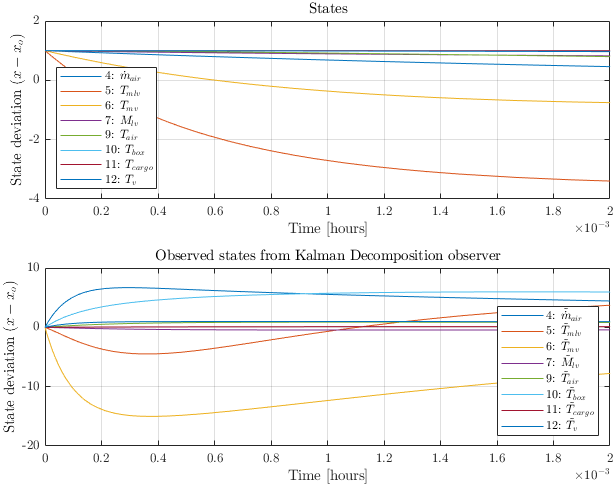
\includegraphics[width=0.66\textwidth]{Graphics/fig_stateObsState002h.png}
	\caption{States and Kalman Decomposition observed states plotted for 0.002 hours. Large deviations observed in the first seconds before observed states converge.}
	\label{fig:sim_stateObsState002h}
\end{figure}

Conclusively the test is a success. The linear state space model simulates and is stable. The Kalman decomposition reduced model used as an observer also performs as hoped and settles onto the states nicely and in timely fashion.
